\documentclass[]{beamer}

\usetheme{Montpellier}
\usecolortheme{rose}

% \usepackage{pgfpages}
% \pgfpagesuselayout{4 on 1}[a4paper, landscape, border shrink=5mm]

\usepackage[utf8]{inputenc}
\usepackage{graphics}
\usepackage{graphicx}
\usepackage{wrapfig}
\usepackage{amsmath}
\usepackage{hyperref}
\usepackage{epstopdf}
 \usepackage{multirow}
 \usepackage[normalem]{ulem}
\bibliographystyle{plain}
\usepackage{color}
\definecolor{BlueViolet} {HTML}{473992}
\definecolor{Marroon}    {HTML}{AF3235}
\definecolor{ForestGreen}{HTML}{009B55}
\definecolor{OliveGreen} {HTML}{3C8031}
\definecolor{fuchsia}    {HTML}{8C368C}

\title{Network Computing courses}
\author{Maël Auzias}
\institute{ENSIBS - UBS}
\date{October 2014}

\AtBeginSection[]  % The commands within the following {} will be executed at the start of each section.
{
\begin{frame} % Within each "frame" there will be one or more "slides."  
\frametitle{Presentation Outline} % This is the title of the outline.
\tableofcontents[currentsection]  % This will display the table of contents and highlight the current section.
\end{frame}
} % Do not include the preceding set of commands if you prefer not to have a recurring outline displayed during your$

\begin{document}

\begin{frame}
  \titlepage
  \begin{figure}[p]
      \centering
      \includegraphics[height=1cm]{./imgs/cc40.jpg}
      \caption{\color{blue}\href{http://teaching.auzias.net}{teaching.auzias.net}}
    \label{fig:cc40}
  \end{figure}
\end{frame}


  \begin{frame}
    \frametitle{Course details}
    \begin{columns}
      \column{.5\textwidth}
        \begin{block}{Objectives}
          \begin{itemize}
            \item How do \emph{computers} communicate?
            \item What are the mechanisms \textbf{under} an HTTP request or a telegram message?
            \item Networks are all around us, better study them!
          \end{itemize}
        \end{block}
      \column{.5\textwidth}
        \begin{figure}[t]
          \centering
          \includegraphics[height=3cm]{./imgs/ntwks.pdf}
          \label{fig:ntwks}
        \end{figure}
    \end{columns}
  \end{frame}

  \begin{frame}
    \frametitle{Course details}
    \begin{columns}
      \column{.3\textwidth}
        \begin{figure}[t]
          \centering
          \includegraphics[height=4cm]{./imgs/grade.pdf}
          \label{fig:marks}
        \end{figure}
      \column{.7\textwidth}
        \begin{block}{Evaluation}
          \begin{itemize}
            \item Short test at the beginning of every lesson (5 min) ?
            \item Project
            \item Final exam (1 hour)
            \item All same weighting
          \end{itemize}
        \end{block}
        \begin{block}{Material}
          \begin{itemize}
            \item Slides available at \color{blue}\href{http://teaching.auzias.net}{teaching.auzias.net} \color{black} (github too)
          \end{itemize}
        \end{block}
    \end{columns}
  \end{frame}


\section{Introduction}
  \begin{frame}
    \frametitle{Definitions and presentation}
      \begin{itemize}
        \item \textbf{Network:} an \textbf{interconnected} group or system\pause
        \item \textbf{Internet:} world wide \textbf{interconnected system of network\emph{s}} \color{blue}\href{http://tools.ietf.org/html/rfc791}{RFC791 (September 1981)}\color{black}\pause
        \item \textbf{IP:} Internet \textbf{Protocol} provides the functions necessary to deliver a package of bits from a source to a destination over a network\pause
        \item \textbf{(world wide) Web:} \textbf{network} consisting of a collection of Internet websites using HTTP
      \end{itemize}
  \end{frame}
  \begin{frame}
    \frametitle{Definitions and presentation}
      \begin{itemize}
        \item \textbf{HTTP:} Hypertext Transfer \textbf{Protocol}, application-level protocol for distributed, collaborative, hypermedia information systems \color{blue}\href{http://tools.ietf.org/html/draft-ietf-httpbis-http2-14}{draft HTTP2 (July 2014)} \color{black}\pause
        \item \textbf{FTP:} File Transfer \textbf{Protocol} promotes sharing of files, encourages the use of remote computers \color{blue}\href{http://tools.ietf.org/html/rfc959}{RFC959 (October 1985)} \color{black} \pause
        \item \textbf{TCP:} Transmission Control \textbf{Protocol} is intended for use as a highly reliable host-to-host \color{blue}\href{http://tools.ietf.org/html/rfc761}{RFC761 (January 1980)} \color{black} \pause
        \item \textbf{UDP:} User Datagram \textbf{Protocol} provides  a procedure  for application  programs  to send messages  to other programs  with a minimum  of protocol mechanism \color{blue}\href{http://tools.ietf.org/html/rfc768}{RFC768 (August 1980)} \color{black} \pause
        \item \textbf{RFC:} Request For Comments (Internet Draft (ID), RFC, Internet Standard)
      \end{itemize}
  \end{frame}
  \begin{frame}
    \frametitle{Definitions and presentation}
      \begin{itemize}
        \item \textbf{Router:} network \textbf{hardware} providing routing services\pause
        \item \textbf{Routing:} \textbf{algorithm processed} to decide where to forward a packet\pause
        \item \textbf{Forwarding:} \textbf{\emph{action}} of moving a packet from one NIC to another\pause
        \item \textbf{NIC:} Network Interface Card
        \item \textbf{Switch (hub):} network \textbf{hardware} connecting systems using packet switching\pause
        \item \textbf{Packet switching:} forward-like method regardless of the content (destination-based)\pause
        \item \textbf{NAT:} Network Address Translation, router modifying IP address into another IP address.
      \end{itemize}
  \end{frame}
  \begin{frame}
    \frametitle{Definitions and presentation}
      \begin{itemize}
        \item \textbf{Node (network):} any entity that can send packets to/receive packets from a network through a NIC\pause
        \item \textbf{Client:} \textbf{computer} able to send requests to a server\pause
        \item \textbf{Request:} \textbf{application message} destined for a server (\emph{order})\pause
        \item \textbf{Server:} \textbf{computer} able to respond a client's requests\pause
        \item \textbf{Response:} \textbf{application message} destined for a client (\emph{result})\pause
        \item \textbf{Fat client:} \textbf{application} where most functions are processed by the client itself\pause
        \item \textbf{Thin client:} \textbf{application} where most functions are carried out on a central server
      \end{itemize}
  \end{frame}

  \begin{frame}
    \frametitle{Network classification}
      \begin{itemize}
        \item \textbf{BAN:} Body Area Network\pause
        \item \textbf{PAN:} Personal Area Networks\pause
        \item \textbf{(W)LAN:} (Wireless) Local Area Networks (home, office, school or airport)\pause
        \item \textbf{MAN:} Metropolitan Area Networks, can cover a whole city\pause
        \item \textbf{WAN:} Wide Area Networks cover a broad area (Internet)
      \end{itemize}
  \end{frame}
  \begin{frame}
    \frametitle{Topologies}
    \begin{figure}[t]
      \centering
      \includegraphics[height=5cm]{./imgs/topologies.png}
      \caption{\color{blue}\href{https://upload.wikimedia.org/wikipedia/commons/thumb/9/97/NetworkTopologies.svg/640px-NetworkTopologies.svg.png}{upload.wikimedia.org}}
      \label{fig:topologies}
    \end{figure}
  \end{frame}
  \begin{frame}
    \frametitle{Topologies}
    \begin{itemize}
      \item \textbf{Point-to-point:} two entities directly connected to each other (tunnel).\pause
      \item \textbf{Ring:} data go around the ring, unidirectional way network.\pause
      \item \textbf{Mesh:} all nodes cooperate in the distribution of data in the network\footnote{\color{blue}\href{http://www.newscientist.com/article/dn26285-hong-kong-protesters-use-a-mesh-network-to-organise.html}{Hong Kong protesters use a mesh network to organize}}.\pause
      \item \textbf{Star:} all messages go through the same central node, reducing network failure.\pause
      \item \textbf{Fully connected:} all nodes are connected to all other nodes.\pause
      \item \textbf{Line:} bidirectional link between two nodes. Node can only send packet going through its neighbors.\pause
      \item \textbf{Bus:} all nodes are connected to the same media. Only one can send a packet at a time, which all others then receive.\pause
      \item \textbf{Tree:} hierarchical topology, such as a binary tree.
    \end{itemize}
  \end{frame}
  \begin{frame}
    \frametitle{Bonus}
    \begin{figure}[p]
      \centering
      \includegraphics[height=3cm]{./imgs/dmanet.pdf}
      \caption{Disconnected MANET illustration \cite{ieee12khabbaz}}
      \label{fig:dmanet}
    \end{figure}
  \end{frame}
  \begin{frame}
    \frametitle{Bonus}
    \begin{figure}[p]
      \centering
      \includegraphics[height=3cm]{./imgs/store-carry-fwd-0.pdf}
      \caption{Store-carry-and-forward \cite{ieee12khabbaz}}
    \end{figure}
  \end{frame}
  \begin{frame}
    \frametitle{Bonus}
    \begin{figure}[p]
      \centering
      \includegraphics[height=3cm]{./imgs/store-carry-fwd-1.pdf}
      \caption{Store-carry-and-forward \cite{ieee12khabbaz}}
    \end{figure}
  \end{frame}
  \begin{frame}
    \frametitle{Bonus}
    \begin{figure}[p]
      \centering
      \includegraphics[height=3cm]{./imgs/store-carry-fwd-2.pdf}
      \caption{Store-carry-and-forward \cite{ieee12khabbaz}}
    \end{figure}
  \end{frame}
  \begin{frame}
    \frametitle{Bonus}
    \begin{figure}[p]
      \centering
      \includegraphics[height=3cm]{./imgs/store-carry-fwd-3.pdf}
      \caption{Store-carry-and-forward \cite{ieee12khabbaz}}
    \end{figure}
  \end{frame}


\begin{frame}
    \frametitle{HTTP request/response example}
      Enter \color{blue}\href{http://getbootstrap.com}{getbootstrap.com} \color{black} in your browser\pause
      \begin{figure}
    \includegraphics[width=11.5cm]{./imgs/dns-req.png}
  \caption{DNS request/response}
      \end{figure}
      \pause
      \begin{figure}
    \includegraphics[trim = 0 0 100mm 0, clip, width=11.5cm]{./imgs/http-req.png}
  \caption{HTTP request/response}
      \end{figure}
  \end{frame}
    \begin{frame}
    \frametitle{How do messages reach their destination?}
      \begin{figure}
    \includegraphics[width=9.5cm]{./imgs/routing.jpg}
  \caption{\color{blue}\href{http://acenk90.files.wordpress.com}{acenk90.files.wordpress.com}}
  \label{fig:routing}
      \end{figure}
  \end{frame}
    \begin{frame}
    \frametitle{More like this...}
      \begin{figure}
    \includegraphics[height=6.5cm]{./imgs/map.jpg}
  \caption{\color{blue}\href{https://upload.wikimedia.org/wikipedia/commons/thumb/d/d2/Internet_map_1024.jpg/768px-Internet_map_1024.jpg}{wikimedia.org}}
  \label{fig:map}
      \end{figure}
  \end{frame}

  \begin{frame}
    \frametitle{Models overview (OSI and TCP/IP)}
    \begin{figure}[t]
      \centering
      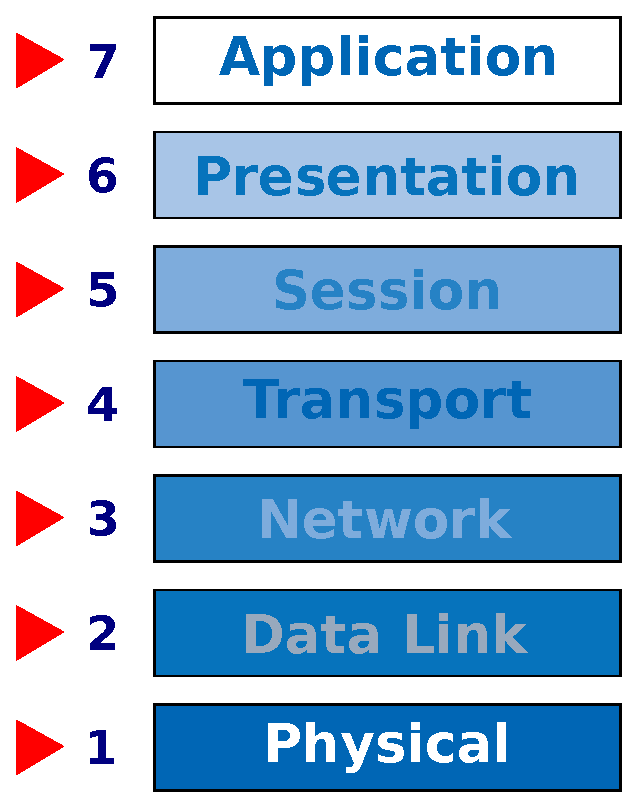
\includegraphics[height=6cm]{./imgs/osi_model.eps}
      \caption{OSI model}
      \label{fig:osi_mod}
    \end{figure}
  \end{frame}
  \begin{frame}
    \frametitle{N\textsuperscript{th} layer communicate with N\textsuperscript{th} layer..}
    \begin{figure}[t]
      \centering
      \includegraphics[height=7.5cm]{./imgs/layer2layer.pdf}
      \caption{layer to layer}
      \label{fig:layer2layer}
    \end{figure}
  \end{frame}
  \begin{frame}
    \frametitle{.. thanks to 3-\textsuperscript{th} layers}
    \begin{figure}[t]
      \centering
      \includegraphics[height=7.5cm]{./imgs/layers_routers.pdf}
      \caption{layers and routing}
      \label{fig:layers_routing}
    \end{figure}
  \end{frame}
  \begin{frame}
    \frametitle{One single protocol, one single layer}
    \begin{figure}[t]
      \centering
      \includegraphics[height=7.5cm]{./imgs/layer2protocol.pdf}
      \caption{protocols and layers}
      \label{fig:layers2proto}
    \end{figure}
  \end{frame}
  \begin{frame}
    \frametitle{Encapsulation}
    \begin{figure}[t]
      \centering
      \includegraphics[height=5cm]{./imgs/encapsulation.pdf}
      \caption{Encapsulation}
      \label{fig:encapsulation}
    \end{figure}
  \end{frame}
\include{1st_layer}
\section{Data Link}
  \begin{frame}
    \frametitle{Aims}
      \begin{itemize}
        \item Interface network layer,\pause
        \item Delivery to unique(?) hardware addresses,\pause
        \item Framing,\pause
        \item Data transfer
      \end{itemize}
  \end{frame}
  \begin{frame}
    \frametitle{Layer composition (of its two sublayers)}
      \begin{enumerate}
        \item Logical Link Control (LLC):
          \begin{itemize}
            \item end to end flow control
            \item end to end error control
            \item (transmitting/receiving) protocols, over MAC sublayer, multiplexing
          \end{itemize}\pause
        \item Media Access Control (MAC):
          \begin{itemize}
            \item physical (hardware) addressing
            \item collision detection and retransmission
            \item data packet scheduling (and queuing)
            \item QoS
            \item VLAN
          \end{itemize}
      \end{enumerate}
  \end{frame}
  \begin{frame}
    \frametitle{Carrier Sense Multiple Access with Collision Avoidance}
    \begin{figure}[t]
      \centering
      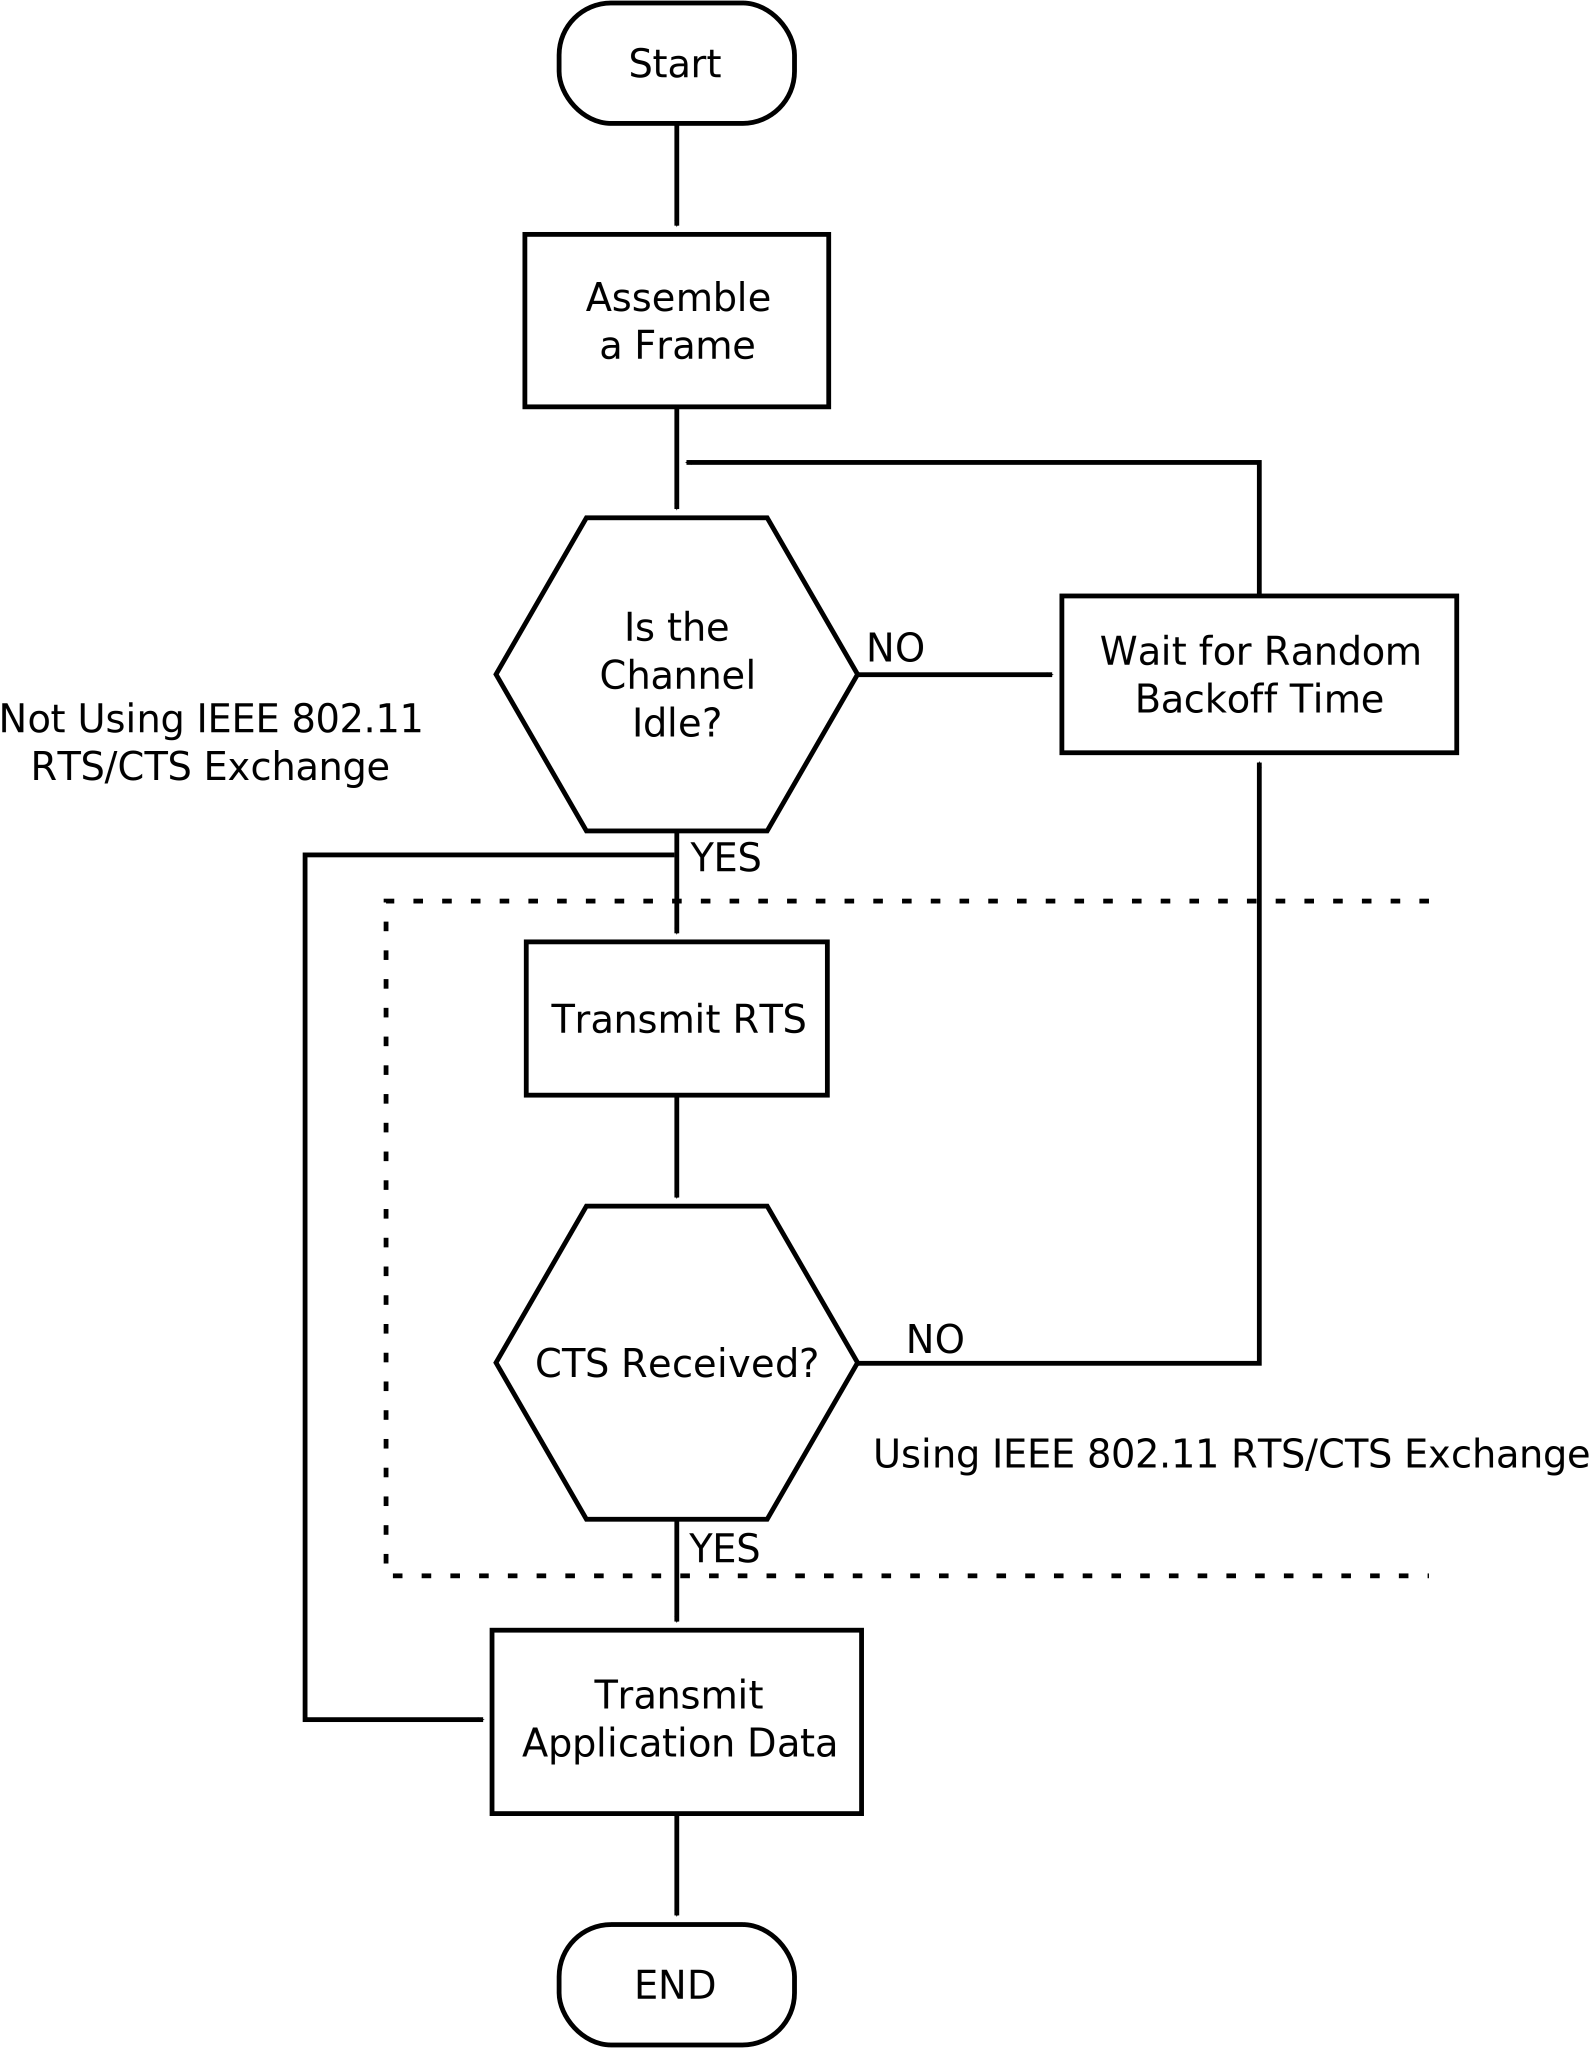
\includegraphics[height=6cm]{./imgs/csma_ca.pdf}
      \caption{\color{blue}\href{https://en.wikipedia.org/wiki/File:Csma_ca.svg}{CSMA CA}}
      \label{fig:csma_ca}
    \end{figure}
    \end{frame}
  \begin{frame}
    \frametitle{Layer 2 Ethernet packet}
      \begin{figure}[h]
      \centering
      \begin{tabular}{|c|c|c|c|c|c|c|c|c|}
        \hline
        \multicolumn{3}{|c|}{MAC dest. (\color{blue}6\color{black})} & \multicolumn{3}{|c|}{MAC src. (\color{blue}6\color{black})} & \multicolumn{2}{|c|}{\color{brown}VLAN tag* (\color{blue}4\color{brown})\color{black}} & Ethertype (\color{blue}2\color{black}) \\ \hline
        \multicolumn{6}{|c|}{Payload (\color{blue}42-1500\color{black})} & \multicolumn{3}{|c|}{Frame check sequence (\color{blue}4\color{black})}\\ \hline
      \end{tabular}
      \caption{Layer 2 Ethernet packet}
      \label{fig:eth_packet}
    \end{figure}
    \hfill \color{brown}optional\color{black}, Content (\color{blue}size in bytes\color{black})
    \begin{figure}[h]
      \centering
      \begin{tabular}{|c|c|}
        \hline
        \textbf{Ethertype 0x} & \textbf{Protocol} \\ \hline
        0800 & IPv4 \\ \hline
        0806 & ARP \\ \hline
        0842 & Wake-on-LAN \\ \hline
        86dd & IPv6 \\ \hline
      \end{tabular}
      \caption{Data received with MDPC}
      \label{fig:eth_type}
    \end{figure}
  \end{frame}


  \begin{frame}
    \frametitle{ARP example}
      \begin{figure}
      \centering
      \resizebox{11.5cm}{!} {
        \begin{tabular}{lcccccccccccccccc}
          \textbf{0000} & ff & ff & ff & ff & ff & ff & fa & ba & 00 & ab & ab & af & 08 & 06 & 00 & 01 \\
          \textbf{0010} & 08 & 00 & 06 & 04 & 00 & 01 & fa & ba & 00 & ab & ab & af & ac & 11 & 22 & 37 \\
          \textbf{0020} & 00 & 00 & 00 & 00 & 00 & 00 & ac & 11 & 00 & f9 & 00 & 00 & 00 & 00 & 00 & 00 \\
          \textbf{0030} & 00 & 00 & 00 & 00 & 00 & 00 & 00 & 00 & 00 & 00 & 00 & 00 \\
        \end{tabular}
      }
      \caption{ARP request}
      \label{fig:arp_packet_ex}
    \end{figure}
        MAC address destination MAC address source Ethertype Hardware type Protocol type OpCode (1 request, 2 reply) IP address source IP address destination
  \end{frame}

  \begin{frame}
    \frametitle{ARP example}
      \begin{figure}
      \centering
      \resizebox{11.5cm}{!} {
        \begin{tabular}{lcccccccccccccccc}
          \textbf{0000} & \color{red}ff & \color{red}ff & \color{red}ff & \color{red}ff & \color{red}ff & \color{red}ff & \color{Marroon}fa & \color{Marroon}ba & \color{Marroon}00 & \color{Marroon}ab & \color{Marroon}ab & \color{Marroon}af & \color{blue}08 & \color{blue}06 & \color{magenta}00 & \color{magenta}01 \\
          \textbf{0010} & \color{OliveGreen}08 & \color{OliveGreen}00 & \color{gray}06 & \color{gray}04 & \color{fuchsia}00 & \color{fuchsia}01 & \color{Marroon}fa & \color{Marroon}ba & \color{Marroon}00 & \color{Marroon}ab & \color{Marroon}ab & \color{Marroon}af & \color{brown}ac & \color{brown}11 & \color{brown}22 & \color{brown}37 \\
          \textbf{0020} & \color{red}00 & \color{red}00 & \color{red}00 & \color{red}00 & \color{red}00 & \color{red}00 & \color{orange}ac & \color{orange}11 & \color{orange}00 & \color{orange}f9 & 00 & 00 & 00 & 00 & 00 & 00 \\
          \textbf{0030} & 00 & 00 & 00 & 00 & 00 & 00 & 00 & 00 & 00 & 00 & 00 & 00 \\
        \end{tabular}
      }
      \caption{ARP request}
      \label{fig:arp_req_ex-colored}
    \end{figure}
    \color{red}MAC address destination \color{Marroon}MAC address source \color{blue}Ethertype \color{magenta}Hardware type \color{OliveGreen}Protocol type \color{fuchsia}OpCode (1 request, 2 reply) \color{brown} IP address source \color{orange} IP address destination
  \end{frame}
  \begin{frame}
    \frametitle{ARP example}
      \begin{figure}
      \centering
      \resizebox{11.5cm}{!} {
        \begin{tabular}{lcccccccccccccccc}
          \textbf{0000} & fa & ba & 00 & ab & ab & af & be & be & 00 & 00 & eb & eb & 08 & 06 & 00 & 01 \\
          \textbf{0010} & 08 & 00 & 06 & 04 & 00 & 01 & be & be & 00 & 00 & eb & eb & ac & 11 & 00 & f9 \\
          \textbf{0020} & fa & ba & 00 & ab & ab & af & ac & 11 & 22 & 37 & 00 & 00 & 00 & 00 & 00 & 00 \\
          \textbf{0030} & 00 & 00 & 00 & 00 & 00 & 00 & 00 & 00 & 00 & 00 & 00 & 00 \\
        \end{tabular}
      }
      \caption{ARP reply}
      \label{fig:arp_rep_ex}
    \end{figure}
        MAC address destination MAC address source Ethertype Hardware type Protocol type OpCode (1 request, 2 reply) IP address source IP address destination
  \end{frame}
  \begin{frame}
    \frametitle{ARP example}
      \begin{figure}
      \centering
      \resizebox{11.5cm}{!} {
        \begin{tabular}{lcccccccccccccccc}
          \textbf{0000} & \color{red}fa & \color{red}ba & \color{red}00 & \color{red}ab & \color{red}ab & \color{red}af & \color{Marroon}be & \color{Marroon}be & \color{Marroon}00 & \color{Marroon}00 & \color{Marroon}eb & \color{Marroon}eb & \color{blue}08 & \color{blue}06 & \color{magenta}00 & \color{magenta}01 \\
          \textbf{0010} & \color{OliveGreen}08 & \color{OliveGreen}00 & \color{gray}06 & \color{gray}04 & \color{fuchsia}00 & \color{fuchsia}01 & \color{Marroon}be & \color{Marroon}be & \color{Marroon}00 & \color{Marroon}00 & \color{Marroon}eb & \color{Marroon}eb & \color{brown}ac & \color{brown}11 & \color{brown}00 & \color{brown}f9 \\
          \textbf{0020} & \color{red}fa & \color{red}ba & \color{red}00 & \color{red}ab & \color{red}ab & \color{red}af & \color{orange}ac & \color{orange}11 & \color{orange}22 & \color{orange}37 & 00 & 00 & 00 & 00 & 00 & 00 \\
          \textbf{0030} & 00 & 00 & 00 & 00 & 00 & 00 & 00 & 00 & 00 & 00 & 00 & 00 \\
        \end{tabular}
      }
      \caption{ARP reply}
      \label{fig:arp_rep_ex-colored}
    \end{figure}
    \color{red}MAC address destination \color{Marroon}MAC address source \color{blue}Ethertype \color{magenta}Hardware type \color{OliveGreen}Protocol type \color{fuchsia}OpCode (1 request, 2 reply) \color{brown} IP address source \color{orange} IP address destination
  \end{frame}
  \subsection{Network}
  \begin{frame}
    \frametitle{Aims}
      \begin{itemize}
        \item Interface transport layer,\pause
	\item Host addressing,\pause
        \item End-to-end packet transmission (data link? Connectionless? Switch? Router?),\pause
        \item Routing, load balancing
      \end{itemize}
  \end{frame}
  \subsubsection{IP addressing}
  \begin{frame}
    \frametitle{Concepts}
      \begin{itemize}
        \item IP addressing fundamentals,\pause
        \item Classfull IP addressing,\pause
        \item Subnet masks,\pause
        \item Variable length subnet masks (VLSM),\pause
        \item Classless inter-domain routing (CIDR).
      \end{itemize}
  \end{frame}

  \begin{frame}
    \frametitle{IP addressing fundamentals}
    \begin{block}{IP address}
      \begin{figure}
        \centering
        \begin{tabular}{|c|c|}
          \multicolumn{2}{c}{32 bits (4x4 bytes)} \\ \hline
           \multicolumn{2}{|c|}{\color{brown}mask} \\ \hline
          \color{brown}Networks part & \color{blue}Host part \\ \hline
        \end{tabular}
        \caption{IP address parts}
        \label{fig:inside_ip_address}
      \end{figure}
    \end{block}
  \end{frame}

  \begin{frame}
    \frametitle{IP addressing fundamentals}
    \begin{block}{Masks}
      \begin{itemize}
        \item Separates network and host bits,\pause
        \item MSB \textbf{always} are ones and then zeros! 255.254.255.0 is not possible,\pause
        \item Indicates how many bits are used for the network part:
        \begin{itemize}
          \item A 8-bit mask leaves 24 bits for the hosts,
          \item A 16-bit mask leaves 16 bits for the hosts,
          \item A 24-bit mask leaves 8 bits for the hosts,
          \item A N-bit mask leaves 32-N bits for the hosts.
        \end{itemize}\pause
        \item Two different mask (differences seen further):
        \begin{itemize}
          \item Network mask,
          \item Subnet mask.
        \end{itemize}
      \end{itemize}
    \end{block}
  \end{frame}
  \begin{frame}
    \frametitle{IP addressing fundamentals}
    \begin{block}{IP address}
      \begin{figure}
        \centering
        \begin{tabular}{|c|c|}
          \multicolumn{2}{c}{32 bits (4x4 bytes)} \\ \hline
          \uncover<2->{\color{brown}ones mask} & \uncover<2->{\color{blue}zeros mask} \\ \hline
          \color{brown}Networks part & \color{blue}Host part \\ \hline
        \end{tabular}
        \caption{IP address parts and mask}
        \label{fig:inside_ip_address_mask}
      \end{figure}
    \end{block}
  \end{frame}

  \begin{frame}
    \frametitle{IP addressing fundamentals}
    \begin{block}{Is that a host?}
      \begin{itemize}
        \item Network address,\pause
        \item Nodes,\pause
        \item Broadcast address.\pause
      \end{itemize}
    \end{block}
    \begin{block}{Within the same network}
      \begin{itemize}
        \item All addresses have the same network bits,\pause
        \item All nodes have different host bits,\pause
        \item Network address has zeros for host bits,\pause
        \item Broadcast address has ones for host bits.
      \end{itemize}
    \end{block}
  \end{frame}

  \begin{frame}
    \frametitle{Example: network 1}
    \begin{figure}
        \centering
      \begin{tabular}{|r|cccc|}
        \hline
        \multirow{2}{*}{Mask /24} & {\color{brown}255} & {\color{brown}255} & {\color{brown}255} & {\color{brown}0} \\
        & {\color{brown}11111111} & {\color{brown}11111111} & {\color{brown}11111111} & {\color{brown}00000000} \\ \hline
        \multirow{2}{*}{Network address} & \color{brown}192 & \color{brown}168 & \color{brown}1 & \color{blue}0 \\
        & \color{brown}11000000 & \color{brown}10101000 & \color{brown}00000001 & \color{blue}00000000 \\ \hline
        \multirow{2}{*}{First nodes address} & \color{brown}192 & \color{brown}168 & \color{brown}1 & \color{blue}1 \\
        & \color{brown}11000000 & \color{brown}10101000 & \color{brown}00000001 & \color{blue}00000001 \\ \hline
        \multirow{2}{*}{Last nodes address} & \color{brown}192 & \color{brown}168 & \color{brown}1 & \color{blue}254 \\
        & \color{brown}11000000 & \color{brown}10101000 & \color{brown}00000001 & \color{blue}11111110 \\ \hline
        \multirow{2}{*}{Broadcast address} & \color{brown}192 & \color{brown}168 & \color{brown}1 & \color{blue}255 \\
        & \color{brown}11000000 & \color{brown}10101000 & \color{brown}00000001 & \color{blue}11111111 \\ \hline
      \end{tabular}
      \caption{IP address example 1}
    \end{figure}
  \end{frame}

  \begin{frame}
    \frametitle{Example: network 2}
    \begin{figure}
        \centering
      \begin{tabular}{|r|cccc|}
        \hline
        \multirow{2}{*}{Mask /16} & {\color{brown}255} & {\color{brown}255} & {\color{brown}0} & {\color{brown}0} \\
        & {\color{brown}11111111} & {\color{brown}11111111} & {\color{brown}00000000} & {\color{brown}00000000} \\ \hline
        \multirow{2}{*}{Network address} & \color{brown}172 & \color{brown}17 & \color{blue}0 & \color{blue}0 \\
        & \color{brown}10101100 & \color{brown}00010001 & \color{blue}00000000 & \color{blue}00000000 \\ \hline
        \multirow{2}{*}{First nodes address} & \color{brown}172 & \color{brown}17 & \color{blue}0 & \color{blue}1 \\
        & \color{brown}10101100 & \color{brown}00010001 & \color{blue}00000000 & \color{blue}00000001 \\ \hline
        \multirow{2}{*}{Last nodes address} & \color{brown}172 & \color{brown}17 & \color{blue}255 & \color{blue}254 \\
        & \color{brown}10101100 & \color{brown}00010001 & \color{blue}11111111 & \color{blue}11111110 \\ \hline
        \multirow{2}{*}{Broadcast address} & \color{brown}172 & \color{brown}17 & \color{blue}255 & \color{blue}255 \\
        & \color{brown}10101100 & \color{brown}00010001 & \color{blue}11111111 & \color{blue}11111111 \\ \hline
      \end{tabular}
      \caption{IP address example 2}
    \end{figure}
  \end{frame}

  \begin{frame}
    \frametitle{Formula}
    \begin{block}{How many \sout{hosts} nodes with a N-bit mask?}
      $2^{32-N}-2$\pause, the $-2$ moves out network and broadcast addresses which are not nodes.\pause
      \begin{itemize}
        \item 24-bit mask: $2^{32-24}-2 = 2^{8}-2 = 254$ nodes \pause
        \item 16-bit mask: $2^{32-16}-2 = 2^{16}-2 = 65.534$ nodes \pause
        \item 8-bit mask: $2^{32-8}-2 = 2^{24}-2 = 16.777.214$ nodes
      \end{itemize}
    \end{block}
  \end{frame}

  \begin{frame}
    \frametitle{Public and private addresses}
    \begin{block}{Public}
      \begin{itemize}
        \item Most of IP addresses \pause
        \item Registered ISP and large organizations inherit blocks of public addresses from IANA\footnote{Internet Assigned Numbers Authority} \pause
        \item Usage of not registered public addresses is forbidden.
      \end{itemize}
    \end{block}
    \begin{block}{Private}
      \begin{itemize}
        \item Privates addresses are A, B and C classes (see after)\pause
        \item No registration needed \pause
        \item Not routed across the Internet \pause
        \item Proxy, NAT and private addresses solved IPv4 shortage.
      \end{itemize}
    \end{block}
  \end{frame}

  
  \begin{frame}
    \frametitle{Classful IP Addressing}
    \begin{figure}
      \centering
      \begin{tabular}{|r||c|c|c|}
        \hline
        Class & A & B & C \\ \hline \hline
        First octet & 1 - 126 & 128 - 191 & 192 - 223 \\ \hline
        First octet pattern 0b& 0* & 10* & 110* \\ \hline
        \multirow{2}{*}{\color{brown}Network mask} & 255.0.0.0 & 255.255.0.0 & 255.255.255.0\\
         & /8 & /16 & /24 \\ \hline
        \multirow{2}{*}{IP addresses range} & 1.0.0.0 & 128.0.0.0 & 192.0.0.0\\
        & 126.0.0.0 & 191.255.0.0 & 223.255.255.0 \\ \hline
        Number of nodes & 16777214 & 65534 & 254 \\ \hline
      \end{tabular}
      \caption{Three main classes}
    \end{figure}
    Where did 127.0.0.0/8 go ?!
  \end{frame}

  \begin{frame}
    \frametitle{Classful IP Addressing}
    \begin{block}{Class D}
      \begin{itemize}
	\item First octet: 224 - 239 \pause
	\item First octet pattern: 1110* \pause
	\item Theses IP addresses are multicast addresses.\pause
      \end{itemize}
    \end{block}
    \begin{block}{Class E}
      \begin{itemize}
	\item Everything left \pause
	\item Experimental class.
      \end{itemize}
    \end{block}
  \end{frame}
  \begin{frame}
    \begin{block}{Reserved addresses}
      \begin{itemize}
	\item 0.0.0.0 used in routing (seen further) \pause
	\item 127.0.0.0/8: loopback addresses (127.0.0.1 - 127.255.255.254).
      \end{itemize}
    \end{block}
  \end{frame}

\section{Transport}
  \begin{frame}
    \frametitle{Aims}
      \begin{itemize}
        \item Interface session layer,\pause
        \item Reliability end-to-end communication,\pause
        \item Order and reassemble received packets,\pause
        \item Flow control,\pause
        \item Congestion avoidance,\pause
        \item Multiplexing
      \end{itemize}
  \end{frame}

  \begin{frame}
    \frametitle{Application identification}
    \begin{block}{Socket address}
      \begin{enumerate}
        \item Node identification is made by IP address,\pause
        \item Application identification is made by node identification..\pause
        \item .. and a port. Number between 0 and 65535. (1-1024: root privilege) \pause
        \item \begin{center} ip.ad.dr.ess:port \end{center}
      \end{enumerate}
    \end{block}
  \end{frame}

  \begin{frame}
    \begin{figure}
      \centering
      \begin{tabular}{l|c}
        Port & Protocol \\ \hline
        21 & FTP \\ \hline
        22 & SSH \\ \hline
        23 & Telnet \\ \hline
        25 & SMTP \\ \hline
        465 & SMTPS \\ \hline
        80 & HTTP \\ \hline
        443 & HTTPS \\ \hline
        3128 - 8080 & Web Proxy \\ \hline
        9418 & git \\ \hline
      \end{tabular}
      \caption{Default port for well known protocol}
      \label{fig:def-port}
    \end{figure}
  \end{frame}

  \begin{frame}
    \frametitle{Socket Primitives (TCP)}
    \begin{figure}
      \centering
      \resizebox{10cm}{!} {
        \begin{tabular}{r|l|l}
          Order & Primitive & Meaning \\ \hline
          1     & SOCKET    & Creates a new communication endpoint \\ \hline
          2     & BIND      & Links local IP address to the socket \\ \hline
          3     & LISTEN    & Signs up for incoming connections \\ \hline
          4     & ACCEPT    & Blocking call till a connection attempt occurs \\ \hline
          -     & CONNECT   & \textbf{Tries} to connect to another communication endpoint \\ \hline
          -     & SEND      & Sends data through the established connection \\ \hline
          -     & RECEIVE   & Receives data through the established connection \\ \hline
          last  & CLOSE     & Releases the connection \\ \hline
        \end{tabular}
      }
      \caption{UDP and TCP primitives}
      \label{fig:primitives}
    \end{figure}
    A socket does not have an IP address until it is bound, just an allocation in the transport entity. A server must listen before any client is able to connect.
  \end{frame}

  \begin{frame}
    \frametitle{}
    %TODO: Frame, Packet, PDU, Datagram, Fragment, + header
  \end{frame}

% \begin{frame}
%   \frametitle{Lessons are going on!}
%   To be continued... ;)
% \end{frame}

%\section*{Conclusion}
%  \begin{frame}
%    \frametitle{References}
%    \bibliography{ref.bib}
%  \end{frame}

\begin{frame}
    \frametitle{Hope you liked it and learnt about networking!}
  \begin{figure}[p]
      \centering
      \includegraphics[height=1cm]{./imgs/cc40.jpg}
      \caption{\color{blue}\href{http://teaching.auzias.net}{teaching.auzias.net}}
    \label{fig:cc40}
  \end{figure}
  \begin{block}{Take a look:}
    \begin{itemize}
      \item "Computer Networks" by A Tanenbaum, Andrew S., G ISBN 013162959X
      \item http://nmap.org/book/toc.html
      \item and many many other resources on the Internet freely available. If you can read it, knowledge is reachable!
    \end{itemize}
  \end{block}
\end{frame}

\end{document}

